\chapter{Alignment}

\section{Task Definition}


One major hurdle in inferring neural structure from EM images is that the image acquisition process is inherently noisy. While the EM imaging technologies used for the creation of neuron images (typically TEM) are quite stable, there is often variance in sample preparation techniques, resulting in all sorts of distortions and errors at imaging time. One particular type of error, image misalignment, occurs during the slicing of sample tissue, when some physical factor causes a resulting slice to be warped or translated in such a way that the resulting stack of images is misaligned. Intuitively, this means that every point in one EM slice data does not necessarily map to the point directly below it the neighboring slice. An example of slice misalignment can be visualized in Figure \ref{fig:misalignment_example}.

\begin{figure}[h]
    \centering
	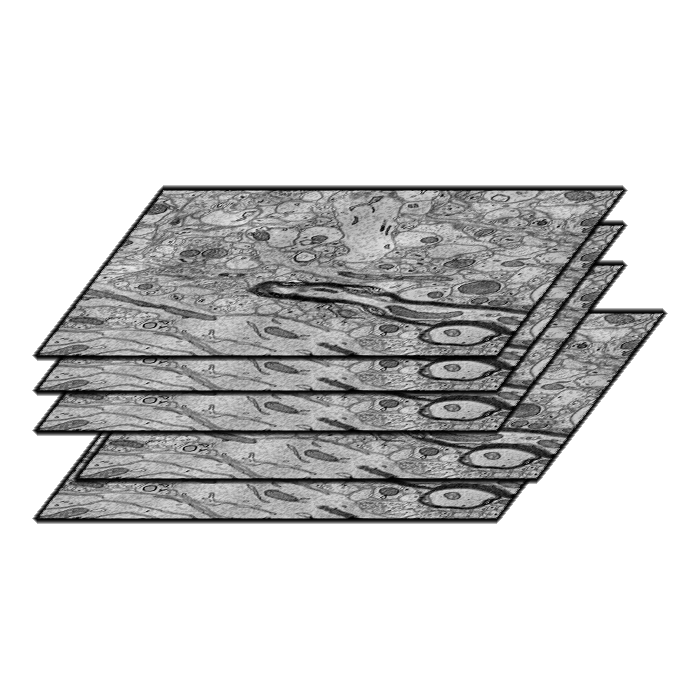
\includegraphics[width=0.33\textwidth]{img/misalignment_example}
	\hspace{1cm}
	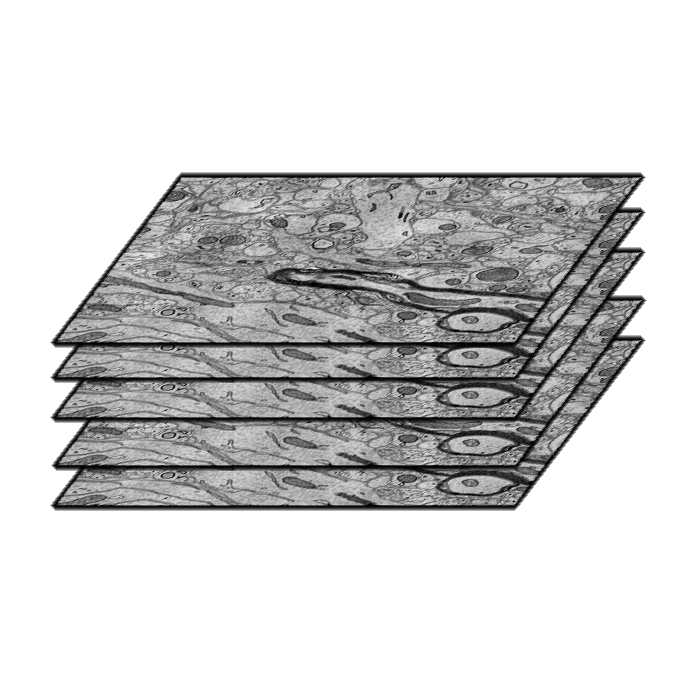
\includegraphics[width=0.33\textwidth]{img/alignment_example}
    \caption[An example of a 3D stack of EM images that contains a misalignment]{An example of a 3D stack of EM images that contains a misalignment. Left: The provided alignment of a stack. This represents a misalignment where the fourth image in a stack of images actually represents a slice slightly translated in position. Right: The correct alignment of the stack, where all the pixels in the fourth position have been translated enough such that the structures depicted in the input data line up in the z-direction.}
    \label{fig:misalignment_example}
\end{figure}

The problem of misalignment within a set of EM images particularly induces problems in the task of 3D Segmentation. While most techniques are rather invariant to small misalignments (particularly CNNs, which can be trained to be invariant to warping of many kinds), large misaligments can often induce false splitting in segmentations. Very deep CNNs trained with a really diverse set of data would likely be able to compensate for these sorts of misalignments, but it would be more prudent to develop a more efficient strategy for automatically healing misalignments in the data. 

\section{Evaluation Metrics}

\section{Models}

\section{Dataset}

\section{Training}

\section{Results}